%
% DSP Report Template
%
% (c) 2005 EMT DSP Group
%
\documentclass[12pt,a4paper]{article}
%\usepackage{dsp_report}

\usepackage{parskip}

%
%\DSPTitle{Odometry for Wheeled Mobile Robots}
%{Michael Maier}

\usepackage{graphicx}

\usepackage{subfigure}
\usepackage{xspace}                   % space nach makro
\usepackage[left]{eurosym}            % Euro symbol
\usepackage{hyperref}

\newcommand{\mbnote}[1]{\textcolor{Gray}{\textbf{\noindent M. Brandner NOTE: #1}}}
\newcommand{\mmnote}[1]{\textcolor{Gray}{\textbf{\noindent M. Maier NOTE: #1}}}
\newcommand{\MH}{\emph{``Mostly Harmless''} RoboCup Team\xspace}
\newcommand{\MSL}{Middle Size League\xspace}
\newcommand{\robocup}{\emph{RoboCup}\xspace}

\begin{document}

%% Based on a TeXnicCenter-Template by Tino Weinkauf.
%%%%%%%%%%%%%%%%%%%%%%%%%%%%%%%%%%%%%%%%%%%%%%%%%%%%%%%%%%%%%

%%%%%%%%%%%%%%%%%%%%%%%%%%%%%%%%%%%%%%%%%%%%%%%%%%%%%%%%%%%%%
%% Deckblatt
%%%%%%%%%%%%%%%%%%%%%%%%%%%%%%%%%%%%%%%%%%%%%%%%%%%%%%%%%%%%%
%%
%% ATTENTION: You need a main file to use this one here.
%%            Use the command "\input{filename}" in your
%%            main file to include this file.
%%
\begin{titlepage}

  \begin{center}
    \begin{minipage}[htb]{18cm}
      \hspace*{-2.6cm}
      
\includegraphics[width=3.3cm]{./figures/logos/LogoEMT.pdf}
      \begin{tabular}{p{10cm}}\centering{
      \Large Institute of Electrical Measurement and Measurement Signal Processing\\ Graz University of Technology
      ~\\
      ~\\}
      \end{tabular}
      
\includegraphics[width=3.3cm]{./figures/logos/TUG.pdf}
    \end{minipage}

    \Large {Bachelor's Thesis\\} %
    \vspace*{1cm} \huge{\textbf{Odometry for Wheeled Mobile Robots}\\}
    %
    \vspace*{1.0cm} 
    %\Huge{\textbf{#1}\\}\vspace*{2.5cm} \vfill
    \Large{Michael Maier\\} \vspace*{1cm}
    %
    \Large{Supervisor: Dipl.-Ing. Dr. Markus Brandner\\} \vspace*{2.5cm}%


    \begin{minipage}[htb]{18cm}
      \hspace*{-0.4cm}
      
\includegraphics[width=3cm]{./figures/logos/MH.jpg}
      \begin{tabular}{p{10cm}}\centering{
        \Large Mostly Harmless RoboCup Team \\Institute for Software Technology, \\Graz University of Technology\\
        \texttt{team@robocup.tugraz.at}\\ \texttt{http://www.robocup.tugraz.at}
        ~\\
        ~\\}
      \end{tabular}
    \end{minipage}

    \Large{Graz, \today}

  \end{center}
\end{titlepage}


\tableofcontents
\clearpage
\pagestyle{plain}


% seitenanzahl dazuschreiben

\begin{abstract}
Abstract

% 1p
\end{abstract}

\clearpage

\section{Introduction}


\subsection{RoboCup}

The RoboCup is an international research and education initiative. 
It's goal is ``By the year 2050, develop a team of fully autonomous robots that can win against the current human soccer world champion team"~\cite{robocup.org}.
It encourages research in the field of robotics, e.g. machine vision, machine learning, autonomous systems.

%|| to Apollo Program.

Every year, a world championship is held accomplished by a conference in a different city around the globe.
Also, various local competitions and conferences are held by local groups.

The RoboCup is divided into three parts: RoboCup Soccer, Rescue and @Home.
Every division is divided into several leagues targeted at different challenges.

%1/2 page

\subsection{\MSL}

In RoboCup Soccer, the \MSL is the most challenging.
The robots have to be fully autonomous.
All sensors, actuators and computation are on board, no external input is allowed.
A Team consists of at most 6~robots with a size of max. $50\times50\times80$\,cm$^3$.

The game is played on a field of $12\times18$\,m$^2$ and lasts $2\times15$~minutes.
The game field surface is usually carpet.
The \MSL is the only league, where an official FIFA ball is used.
Objects are distinguished by colour, the game field is green with white lines, robots and referees are black and the ball is red.

The rules are official FIFA rules~\cite{msl-rules} with slight adaptions for robotic players.
The game rules are tightened every year to keep up with the technological progress. 
E.g. the field size has grown from $6\times8$\,m$^2$ to $12\times18$\,m$^2$ since introduction of the \MSL.

More than 20 teams from all over the world participate in the \MSL, almost all with academical background.

% 1/2 p

\subsection{\MH}

The \MH participates in the \MSL. 
It's name is a reference to the ``Hitchhiker's Guide to the Galaxy'' by Douglas Adams~\cite{h2g2}.
It was founded 2003 at Graz University of Technology at the Institute for Software Technology. 
It consists solely of students and acts as a platform for master's, bachelor's thesis and seminar projects.
Currently, more than 30~students are working on the robots in their free time.

It regularly participates at European championships as well as World Championships.
RoboCup 2009 in Graz was the first time the team advanced a round in a World Championship. 
Also, the third place in the technical challenge was won.



% 1/4 p

\subsection{Current Robot Platform: Krikkit}

The ``Krikkit'' robot platform was built in 2006~\cite{}. 
It was designed solely for playing soccer, in contrast to the old, multi-purpose research robot platform.
Nearly all components, from electronics to mechanical parts are developed in-house.
Four robots were built and made their debut at the World Championship 2006 in Bremen.

Some of the main features of the ``Krikkit'' robot are shown in \autoref{fig:krikkit}.

\begin{figure}[ht]
\begin{center}
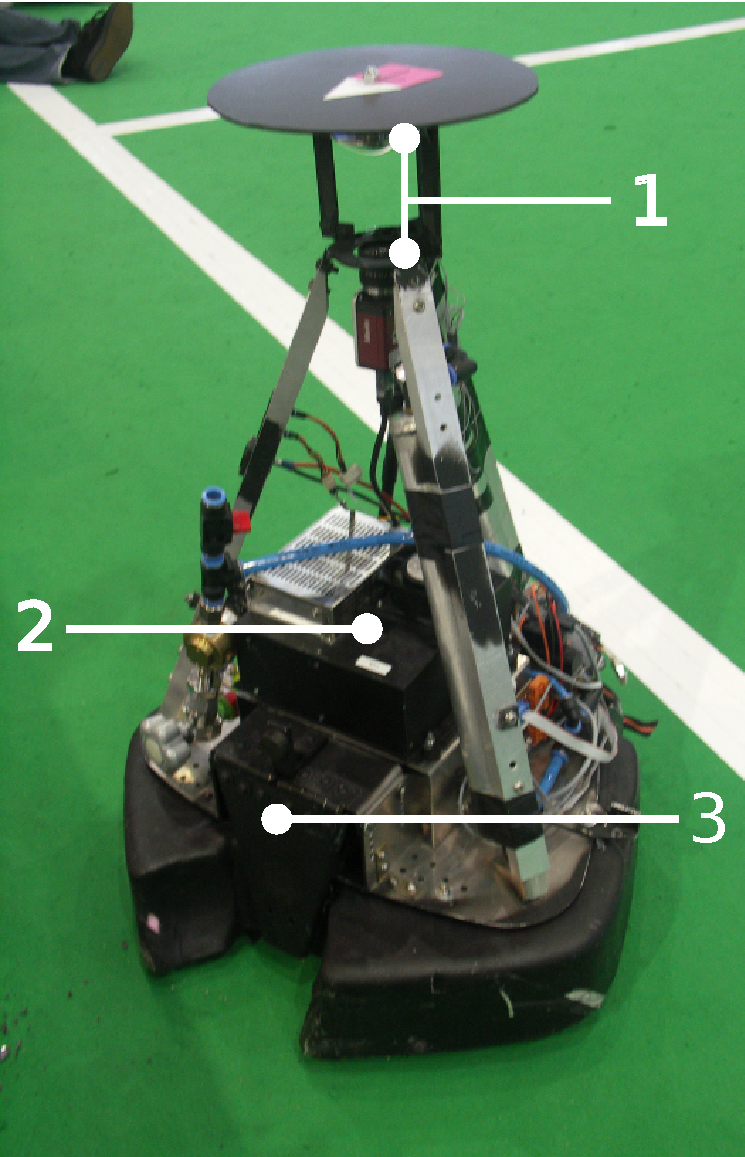
\includegraphics[width=0.5\columnwidth]{figures/krikkit.pdf}
\caption{\label{fig:krikkit}
Krikkit robot. Omnivision with camera and mirror~(1); Industrial PC~(2); Pneumatic kicker~(3); Omnidrive is below the black bumper.
}
\end{center}
\end{figure}

It has a $360^\circ$ omnidirectional vision system via a firewire-camera pointing upwards to a hyperbolic mirror.\\
Its brain is a standard mini-ITX industrial PC.\\
A powerful pneumatic kicker with a~200\,bar pressurised air bottle as supply enables the robot to kick the ball approx. 10\,m forward.\\
Its drive system is also omnidirectional and is based on self-designed Mecanum wheels~\cite{mecanum2007}. 
The $45^\circ$-Arrangement of the wheels (see~\autoref{fig:mec-wheel}) promised smooth and vibration-free operation.
The three wheels are arranged in $120^\circ$-steps (see~\autoref{fig:omnidrive}) and are driven by a 200\,W brushless DC motor for each axis.
Due to the nature of omni-wheels, the robots are able to move in any direction and any orientation.\\
The motors and all other electric components are supplied by a smart battery system~\cite{krammer06}.
All electronic components are connected via CAN-Bus.

\begin{figure}[hb]
  \begin{minipage}{0.45\textwidth}
   \centering
    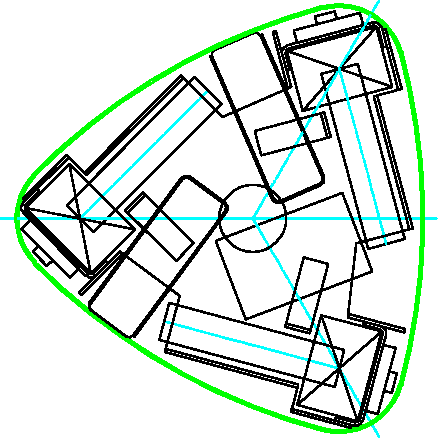
\includegraphics[width=1\textwidth]{figures/krikkit_drive}
    \caption{\label{fig:omnidrive}Omnidrive \cite{mecanum2007}}
  \end{minipage}\hfill
  \begin{minipage}{0.45\textwidth}
   \centering
    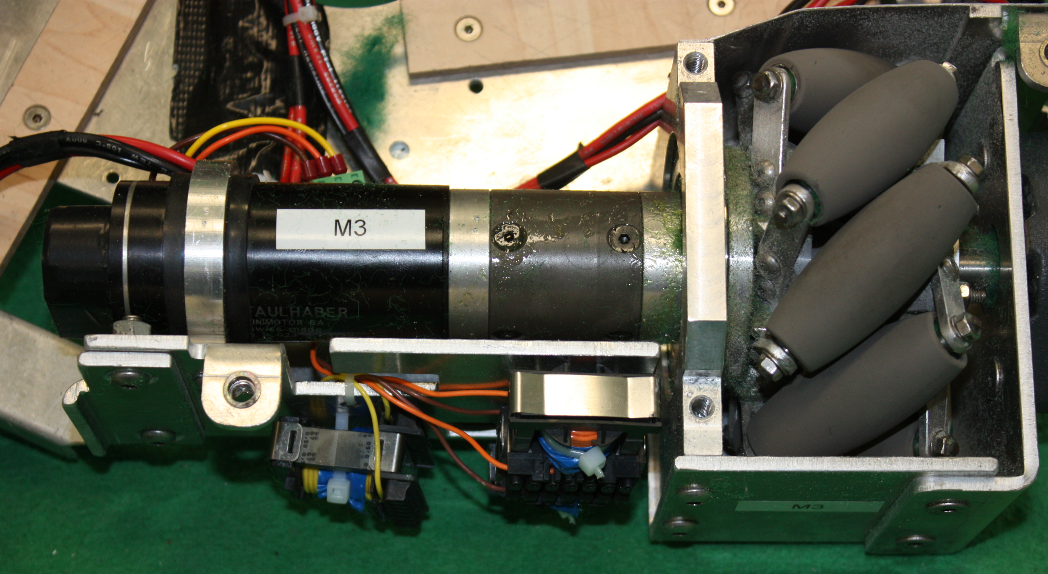
\includegraphics[width=1\textwidth]{figures/Omniwheel_drive.png}
    \caption{\label{fig:mec-wheel}Mecanum wheel with motor and gearbox.}
  \end{minipage}
\end{figure}


The Krikkit robots served well for four years, much was learned.
Before RoboCup~2009 in Graz, a major mechanics overhaul was done.
In the meantime, all major electronic components also reached the end of their life cycle.
With the knowledge gained, lost and acquired again the successor of the Krikkit generation is in development now.
    

\subsection{In Development: Krikkit3G}

The next generation of robots is in development since mid-2010.
It will be a direct successor of the Krikkit generation, therefor the name \emph{Krikkit3G}.
The successful concepts are are adopted nearly unchanged:

\begin{itemize}
  \item omnidrive with the three Mecanum Wheels
  \item the omni-vision system
  \item pneumatic kicking concept
  \item the use of a standard mini-ITX industrial PC
  \item modularity of all components
\end{itemize}

The new robot design focuses on the strict modularity of all components.
It has been shown that fast disassembling and replacing of critical components is crucial in the fast-paced tournament environment.
Especially the power train has been modularised, the wheel, gearing, motor and motor electronics can be swapped as a whole group.

Tests showed that the smoothness of the Mecanum wheels was insufficient due to manufacturing imprecision.
The resulting vibrations should be filtered out by an independent wheel suspension.

%  bumpers ?

For the kicking system, the pneumatic principle was kept.
But it is now much more versatile. 
It can switch between high and flat kicks at full power, and side-kicks are also possible now.
It features a new ball guidance system, which allows grabbing the ball for a short moment.
This becomes especially useful when decelerating.

Big changes were made in the electronics sector.
A new microcontroller core (An ARM Cortex~M3) is used on every component, replacing the different microcontroller architectures used before.
The smart battery system also got a major upgrade, featuring even smarter batteries.

In the mechanical design, space is now also provided for an improved odometry system, which will be developed based on this work.


\begin{figure}[b]
\begin{center}  
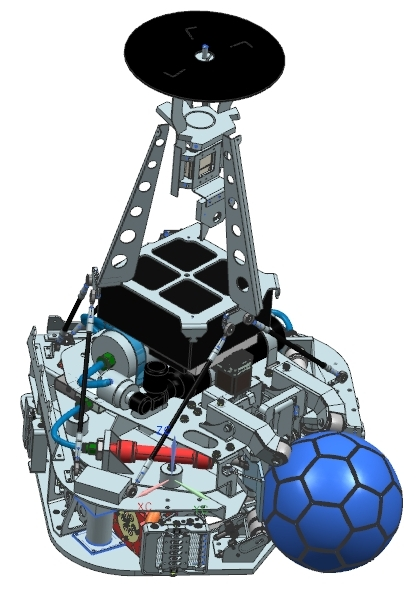
\includegraphics[width=0.5\columnwidth]{figures/Krikkit3G.jpg}
\caption{\label{fig:krikkit3g}
Rendering of the Krikkit3G robot.
}   
\end{center}
\end{figure}


% 1p

\subsection{Motivation for this Work}
  
Current odometry systems of the Krikkit generation is based on the rotational speed of the wheels.
This has the major disadvantage of the accurancy bound to the slip of the wheels.
The problem is the nonuniform structure of the game field carpet, which has different slip factors in each direction.
Due to the different speeds and angles of the Mecanum wheels, this leads to deviations even when driving a straight line.
The errors accumulate over time, resulting in $90^\circ$~deviation on 10\,m straight distance driven.

Therefor, an wheel-independent odometry system has to be developed.
The goal of this work was:

\begin{itemize}
  \item Gathering requirements for a sensor
  \item Search for different types of sensors
  \item Implementation and validation of a prototype
\end{itemize}



%Motivation and Goal

%1/2p

%chaptersum 5p

\clearpage
\section{Odometry}
%  Definition
%  Verwendungsmoeglichkeit
%    Lokalisierung
%      higher framerate than cam
%      backup-system for cam
%    Motion control
%      anti-slip regulation

Odometry, better known as path measurement is important for every moving vehicle, especially robots which need to know where they currently are. 


1p

\subsection{Odometry Measurement}

\subsubsection{Current Implementations used}

      wheel encoder
        probleme
      2. satz raeder
        probleme

1p

\subsubsection{Possible Implementations}

      radar
1/4
      accelerometer
        2G spitzenvibration -> no
1/4
      Ultrasonic Doppler Velocimetry
1/4
      Microwave Doppler Velocimetry
1/4
      Laser interferometry
1/2
      Optical Spatial Frequency Filtration
1/4
        Daniel's approach
1/4
        laser speckle applications
        optical mice
1/2

3p

sum 4p

\subsection{Requirements for a new type of Odometry Sensor on the Krikkit/3G platform}

1p


\subsection{Decision for a Type of Sensor}
  entscheidung fuer einen Sensortyp
    - why/why not...
    - ...
    - ...

1p


chaptersum 8p

\section{Designing the Sensor for Evaluation}

block diagram
  ADNS + optic
  XC
  PC

1p

\subsection{The ADNS 6010}

specs

workflow diagram (from datasheet)

1p

\subsubsection{Custom PCB}
ADNS-testplatine
  requirements

  circuit diagram

  PCB drawing

2p

sum 4p
  
\subsection{Optical System}
  requirements

1/2p

\subsubsection{Original Mouse Setup}

1p

\subsubsection{2-Lens Setup}

1p

\subsubsection{Telecentric Setup}

1p

sum 4p
\subsection{The XC164 Microcontroller}

Specs etc

XC-164 eval board 
  Image from datasheet

1/2p

\subsubsection{Wiring of the Evaluation Board}

  block diagram

  circuit

1p

\subsubsection{uC - Software}

  XC-Code
    requirements
    firmware catch

    image streaming

    motion data streaming
      + reference sensor

4p

sum 6p


\subsection{Data Acquisition Software}

\subsubsection{PyQT GUI}
1p

\subsubsection{Octave Analysis Scripts}
1/2p


sum 2p

chaptersum 17p

\section{Experimental Setup}

- requirements

1p

\subsection{Mechanical Design of the Testbed}

block diagram

1p

\subsection{Optical System}

micro-bench system

Sketch

1/2p

\subsubsection{Sensor mounting \& Calibration}

Sketch with adjusting screws in all dimensions

1/2p

calibration process
  laser

1p

\subsubsection{Lens 2 \& Aperture Mounting}

manufacturing drawing

1p

\subsubsection{Illumination}

  Why here?
  types of LEDs and Lasers used
 
  Illumination PCB

  circuit

  PCB print

2p

\subsection{Motor \& Disk}

1/2p

\subsection{Reference Speed Sensor}
      Picture of sensor from Datasheet
      electrical setup used

1p

\subsection{Microcontroller \& Host PC}      

1/2p


chaptersum 9p

\section{Experimental results}

\subsection{Illumination tests}

\begin{itemize}
  \item Laser
  \item Studio Spotlight
  \item ultra-bright white LEDs
  \item IR-LEDs
\end{itemize}

\subsection{Non-telecentric tests}

\subsection{Telecentric tests}

\subsubsection{Carpet 1}

\subsubsection{Carpet 2}

\subsubsection{Carpet 3}

\subsubsection{Game Field Lines}

\subsection{Interpretation}

  plots
  ergebnisse

groesser 5p

\section{Outlook - Next Steps}

  evaluation of a combination of IR-LED illumination and Laser illumination

  newer sensor ADNS-90xx

  mechanical limitations
    size constraints
    dirt cleaning...
  electrical requirements
    new architecture: ARM
    also include illumination control in uC
      use of the shuttered illumination for higher power 
      use of both LEDs and Lasers for white lines
  software algorithms: compute 3 dimension out of 2/4/6

ca 3-5p


summe gesamt 49 Seiten (ohne abstract, inhaltsv, bibl.)


%--------------------------------------------------------%
% Bibliography
%--------------------------------------------------------%
\addcontentsline{toc}{section}{Bibliography}
\label{Bibliography}
\bibliographystyle{plain}
\bibliography{literature}
%
\end{document}
